\documentclass{article}

\usepackage{tocloft}
\usepackage[top=2.5cm, bottom=2.5cm, left=2.2cm, right=2.2cm]{geometry}
\usepackage{graphicx}
\usepackage[localise,Kashida]{xepersian}

\renewcommand{\cftsecleader}{\cftdotfill{\cftdotsep}}
\settextfont{Vazir}

\begin{document}

\setLTRbibitems{}

\نویسنده{الهه داستان}
\عنوان{طراحی و پیاده‌سازی سیستم پیش‌بینی ترافیک بر پایه شبکه‌های عصبی}
\تاریخ{\امروز}
\عنوان‌ساز
\فهرست‌مطالب

\قسمت{تعریف مساله}
\پاراگراف{}
پیش‌بینی سرعت ترافیک برای کنترل و هدایت آن ضروری است.
به علت پیچیدگی و غیرخطی بودن جریان ترافیک روش‌های قدیمی نمی‌توانند ترافیک را برای سفرهایی با زمان طولانی و متوسط به خوبی پیش‌بینی کنند.
پیش‌بینی دقیق و بی‌درنگ سرعت ترافیک برای افراد و سازمان‌های ارائه دهنده‌ی خدمات حمل و نقل و حتی دولت موضوع مهمی است چرا که حمل و نقل نقش مهمی در زندگی هر فرد ایفا می‌کند و یکی از اصلی‌ترین توانایی‌ها در سیستم ترابری هوشمند \پانویس{Intelligent Transportation System} به شمار می‌رود.
در این پروژه سعی داریم با استفاده از آموزش دادن شبکه‌های عصبی عمیق به پیش‌بینی سرعت ترافیک در برخی نقاط مشخص (مانند چهارراه‌ها و میدان‌ها) بپردازیم.
امروزه با استفاده از داده‌های عظیمی که در دسترس است و همچنین پیشرفت سخت‌افزار می‌توانیم شبکه‌های عمیقی که در گذشته قابل آموزش نبودند را آموزش دهیم و از توانایی بالای آن‌ها در پیش بینی مسائل پیچیده استفاده کنیم.

\قسمت{مرور پیشینه}
\پاراگراف{}
پیش‌بینی سرعت ترافیک بر مبنای طول سفر به دو دسته‌ی کلی کوتاه (۵ تا ۳۰ دقیقه) ‌و متوسط-طولانی (بیشتر از ۳۰ دقیقه) تقسیم می‌گردد. اکثر روش‌های آماری مانند رگراسیون خطی در سفرهای کوتاه مدت عملکرد خوبی دارند، اما به علت عدم قطعیت و پیچیدگی جریان ترافیک این روش‌ها در سفرهای طولانی مدت دقت خوبی ندارند.~\مرجع{1709.04875}

\پاراگراف{}
مطالعات قبلی بر روی پیش‌بینی سرعت ترافیک در سفرهای بلند مدت را می‌توان به دو دسته‌ی مدل کردن پویا و روش‌های داده‌محور تقسیم کرد.
در روش‌های مدل کردن پویا از ابزار ریاضیاتی، مانند معادلات دیفرانسیل و دانش فیزیکی، برای فرموله کردن مسائل ترافیک استفاده می‌شود.~\مرجع{Vlahogianni2015}
در این روش برای رسیدن به حالت پایدار در پروسه‌ی شبیه‌سازی به سیستم‌های پیچیده و توانایی محاسباتی بسیار بالا نیاز است و فرضیه‌ها برای ساده‌سازی، دقت پیش‌بینی را کاهش می‌دهند.
به همین دلت و همانطور که پیشتر بیان شد، به دلیل وجود داده‌ی زیادی که امروزه قابل دسترس است، علاقه به سمت روش‌های داده محور بیشتر است.
در روش‌های داده محور مدل‌های آماری کلاسیک و مدل‌های یادگیری ماشین دو نماینده‌ی اصلی هستند.

\پاراگراف{}
روش مدل خود همبسته میانگین متحرک\پانویس{Auto-Regressive Integrated Moving Average} و انواع آن یکی از روش های تجزیه و تحلیل سری زمانی است که مبتنی بر آمار کلاسیک\پانویس{Classical Statistics} است
و در طول زمان بسیار مورد بحث قرار گرفته است~\مرجع{Williams2003}،
اما این مدل محدود به فرضیات ثابتی درباره‌ی توالی‌های زمانی است و نمی‌تواند ارتباطات زمانی-مکانی را به حساب بیاورد.
اخیرا روش‌های یادگیری ماشین در پیش‌بینی سرعت ترافیک توانسته‌اند مدل‌های آماری کلاسیک را به چالش بکشند.

\پاراگراف{}
امروزه روش‌های یادگیری عمیق با موفقیت بر روی مسايل ترافیکی اعمال شده‌اند و پیشرفت‌های زیادی در این زمینه صورت گرفته است،
مانند شبکه‌ی باور عمیق\پانویس{Deep Belief Network}~\مرجع{YuhanJia2016} و کدکننده خودکار پشته‌ای\پانویس{Stacked Auto Encoder}~\مرجع{Chen_Song_Yamada_Shibasaki_2016}.
اما برای این شبکه‌های متراکم سخت است که بتوانند ویژگی‌های زمانی و مکانی را به طور مشترک از ورودی استخراج کنند.
همچنین در هنگام محدودیت و یا غیبت ویژگی‌های مکانی توانایی این شبکه‌ها تحت تاثیر قرار میگیرد.

\قسمت{راه‌حل پیشنهادی}

\پاراگراف{}
برای درک بهتر موضوع همزمان با توضیح راه‌حل یک مثال را به طور موازی پیش می‌بریم.

\پاراگراف{}
هدف از این پروپوزال بیان راه‌حلی برای پیش‌بینی سرعت ترافیک در برخی مختصات‌ها (مانند تعدادی میدان) در چند گام زمانی آینده است که
بدین جهت از سرعت ترافیک در این محل‌ها در گام‌های زمانی پیشین استفاده می‌کنیم. رابطه \رجوع{eq:base} این مساله سری زمانی را به زبان ریاضی توصیف می‌کند.

\begin{equation}
  \label{eq:base}
  \hat{v}_{t+1}, \ldots,  \hat{v}_{t+H} = \mathop{\mathrm{argmax}} \log \mathsf{P}({v}_{t+1}, \ldots,  v_{t+H} | v_{t-M+1} , \ldots,  v_{t})
\end{equation}

\begin{table}[h]
  \centering
  \caption{توضیح پارامترهای رابطه \رجوع{eq:base}}
  \begin{tabular}{|c|p{0.5\textwidth}|}
    \hline
    $v_{t}$ & یک بردار به طول تعداد نقاطی که قصد داریم سرعت ترافیک را در آن‌ها پیش‌بینی کنیم که هر المان شامل سرعت ترافیک در یکی از مختصات‌های مورد نظر در زمان $t$ است. \\
    \hline
    $\hat{v}_{t+1}$ & سرعت پیش‌بینی شده در زمان $t+1$ \\
    \hline
    $H$ & تعداد گام های زمانی آینده که می خواهیم سرعت ترافیک را پیش بینی کنیم. \\
    \hline
    $M$ & تعداد گام های زمانی پیشین که برای پیش بینی استفاده می کنیم. \\
    \hline
  \end{tabular}
  \label{tbl:base}
\end{table}

\پاراگراف{}
برای مثال فرض کنیم می‌خواهیم سرعت ترافیک را در میدان فاطمی و میدان فلسطین (دو میدان معروف در تهران) پیش‌بینی کنیم.
$v_{t}$ یک بردار به طول دو خواهد بود که یک عضو آن سرعت ترافیک در میدان فاطمی در زمان $t$ مانند ساعت دو بعد از ظهر امروز و عضو دیگر آن شامل همین اطلاعات برای میدان فلسطین خواهد بود.
در این مثال $H$ را برابر یک و $M$ را برابر سه در نظر می گیریم. منظور از \رجوع{eq:base} این است که می‌خواهیم سرعت ترافیک در $H$ قدم زمانی بعدی را با دانستن $M$ قدم زمانی قبلی پیش‌بینی کنیم
در این مثال اگر اندازه‌ی گام زمانی را برابر یک ساعت فرض کنیم، می‌خواهیم سرعت ترافیک در یک ساعت بعدی را با توجه به سه ساعت قبل پیش‌بینی کنیم.

\پاراگراف{}
برای پیش‌بینی سرعت ترافیک در نقاط مختلف از هر دو نوع ویژگی زمانی و مکانی بهره می‌بریم.
در روش‌های پیشین مانند \مرجع{1506.04214} از پیچش معمول که عمدتا در پردازش تصویر از آن بهره می‌گیرند استفاده شده است، این پیچش تنها می‌تواند بر روی داده‌هایی اعمال شود که ساختار مشبک دارند (مانند عکس و فیلم).
در این روش برای آنکه بتوانیم از اطلاعات مکانی حداکثر استفاده را ببریم به جای آنکه شبکه‌ی ترافیک را مانند یک شبکه‌‌ی شطرنجی\پانویس{Grid} ببینیم،
آن را به وسیله‌ی یک گراف مدل می‌کنیم و پیچش را مستقیما بر روی این گراف اعمال می‌کنیم.

\پاراگراف{}
گره‌های این گراف نقاطی مشخص هستند که سرعت ترافیک را در آن‌ها داشته باشیم که در این مثال نقاط ما میدان‌های فاطمی و فلسطین هستند،
سرعت در این نقاط به طور مثال می‌تواند از طریق دوربین‌های سرعت سنج یا از طریق سیستم موقعیت‌‌یاب‌جهانی\پانویس{GPS} رانندگان تشخیص داده شود.

\پاراگراف{}
رابطه \رجوع{eq:base} را به صورت شهودی می‌توان به وسیله‌ی شکل \رجوع{fig:base} نشان داد.

\begin{figure}
  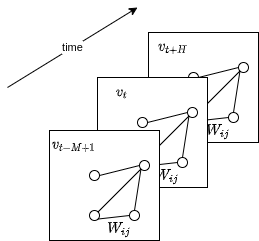
\includegraphics{./images/base.png}
  \centering
  \caption{
گراف مسیر یکسان است و هر دیاگرام نشان دهنده‌ی جریان ترافیک در گره‌های این گراف در یک لحظه متفاوت است
  }
  \label{fig:base}
\end{figure}

\پاراگراف{}
بدیهی است تغییر سرعت ترافیک در یک گره‌ی گراف می‌تواند باعث تغییر سرعت ترافیک در گره‌های مجاور شود و هر چه فاصله‌ی دو گره از یک دیگر کم تر باشد این اثرگذاری قوی‌تر است.
برای نمایش این عامل به صورت کمی از ماتریس $W$ استفاده می‌کنیم، ابعاد این ماتریس به صورت $n x n$ است که $n$ برابر تعداد گره‌های گراف است و هر مقدار داخل این ماتریس نشان دهنده‌ی میزان انتشار تغییرات سرعت بین دو گره متناظر با توجه به فاصله‌ی مکانی آن‌ها است.

\پاراگراف{}
در شکل \رجوع{fig:base} $W_{i,j}$ نشان دهنده‌ی میزان ارتباط مکانی و همبستگی بین گره‌های $i$ و $j$ است در این مثال گره‌های $i$ و $j$ همان میادین یاد شده هستند و $W_{i,j}$ با توجه به فاصله ی مکانی این دو میدان نشان می‌دهد که
به طور مثال اگر سرعت ترافیک در میدان فاطمی کاهش پیدا کند این موضوع چقدر می‌تواند بر روی سرعت ترافیک در میدان فلسطین تاثیر بگذارد.
در این پروژه از رابطه‌ \رجوع{eq:distance} برای به دست آوردن آن‌ها استفاده می‌کنیم \مرجع{1709.04875}:

\begin{equation}
  W_{i,j} = \left\{
    \begin{array}{ll}
      \exp(-\frac{d^{2}_{ij}}{\sigma^{2}}) & , i \neq j \quad and \quad \exp(-\frac{d^{2}_{ij}}{\sigma^{2}}) \geq \epsilon \\
      0 & , otherwise. \\
    \end{array}\right.
  \label{eq:distance}
\end{equation}

\begin{table}[h]
  \centering
  \caption{توضیح پارامترهای رابطه \رجوع{eq:distance}}
  \begin{tabular}{|c|p{0.5\textwidth}|}
    \hline
    $W_{ij}$ & میزان ارتباط مکانی بین گره‌های $i$ و $j$ \\
    \hline
    $d_{ij}$ & فاصله ی مکانی بین گره‌های $i$ و $j$ \\
    \hline
    $\sigma$, $\epsilon$ & پارامترهای ثابت برای کنترل میزان تنک\پانویس{Sparsity} بودن ماتریس $W$ \\
    \hline
  \end{tabular}
  \label{tbl:distance}
\end{table}

\پاراگراف{}
در مثال ما فاصله بین میدان‌های فاطمی و فلسطین برابر ۱.۷ کیلومتر است.
هرچه $\epsilon$ را افزایش دهیم باعث می‌شود تنها ارتباطات قوی‌تر را به حساب بیاوریم و ماتریس تنک‌تر می‌شود
همچنین هرچه $\sigma$ را کاهش دهیم عددی که به عنوان میزان ارتباط محاسبه می‌کنیم کاهش یافته و ماتریس تنک‌تر می‌شود.

\پاراگراف{}
با توجه به توضیحات بالا برنامه به دو فایل ورودی احتیاج دارد که اطلاعات درج شده در شکل \رجوع{fig:blackbox} را در اختیار برنامه قرار دهند.
در فایل اول گراف یا به عبارتی وزن یال‌ها شرح داده می‌شود $W$ و در دیگری سرعت ترافیک در نودها در بازه‌های زمانی متوالی قرار می‌گیرد $(v_{t}, \ldots, v_{t-M+1})$.
در خروجی جریان ترافیک پیش‌بینی شده در نودها در قدم زمانی بعدی به ما گفته می‌شود $\hat{v}$. در مثال ما فایل‌های ذکر شده فرمتی مانند جدول  دارند البته اعداد زیر به صورت تصادفی و فرضی هستند.

\begin{figure}
  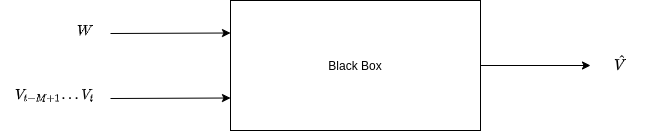
\includegraphics{./images/blackbox.png}
  \centering
  \caption{
در یک نگاه سطح بالا برنامه با دانستن گراف و جریان ترافیک در گره های این گراف در M واحد زمانی گذشته جریان ترافیک در واحد زمانی بعدی را تخمین زده و برمی‌گرداند.
  }
  \label{fig:blackbox}
\end{figure}

\پاراگراف{}
برای سادگی گراف را بدون جهت در نظر می‌گیریم و در نتیجه $W$ ماتریسی متقارن است.

\پاراگراف{}
بلوک‌های تشکیل دهنده‌ی نرم افزار را در شکل \رجوع{fig:block} مشاهده می‌کنید، ساختار برنامه از دو بلوک پیچشی زمانی-مکانی و یک لایه‌ی خروجی کاملا متصل در انتها تشکیل شده است.

\begin{figure}
  \includegraphics{./images/block.png}
  \centering
  \caption{
شبکه‌ی کانولوشنی زمانی-مکانی بر روی گراف \مرجع{1709.04875}
  }
  \label{fig:block}
\end{figure}

\bibliographystyle{ieeetr}
\bibliography{references}

\end{document}
